\documentclass[a4paper,11pt,dvipdfmx]{jsarticle}


% 数式
\usepackage{amsmath,amsfonts}
\usepackage{bm}
% 画像
% \documentclass{article}
\usepackage[dvipdfmx]{graphicx}
\usepackage{circuitikz}
\usepackage{amsmath,amssymb}
\usepackage{siunitx}
\usepackage{float}
\usepackage{tikz}
\usepackage{askmaps}
\usepackage{multirow}
\usepackage{bigstrut}
\usepackage{slashbox}
\usepackage{rotating}

\begin{document}


\newpage
\section{目的}
電子天秤の制作を行うにあたり、値を表示させるために7セグメントLED1の表示回路を作成する。デコーダ回路の入力は、セレクタ回路から3bitの信号を受け取る。
\section{原理}
実際に回路の制作を行うにあたって使用する部品と動作原理を説明する。
\subsection{ブレッドボード}
ブレッドボードを使用し、デコード回路の作成を行う。この部品はジャンパ線を使用して自由に回路を組み替えれるので、回路の制作に適している。
ブレッドボード上で配線するときはショートしているピンについて理解をしないといけない。
図\ref{fig:breadboard}にブレッドボード写真を示す。
\begin{figure}[h]
  \centering
  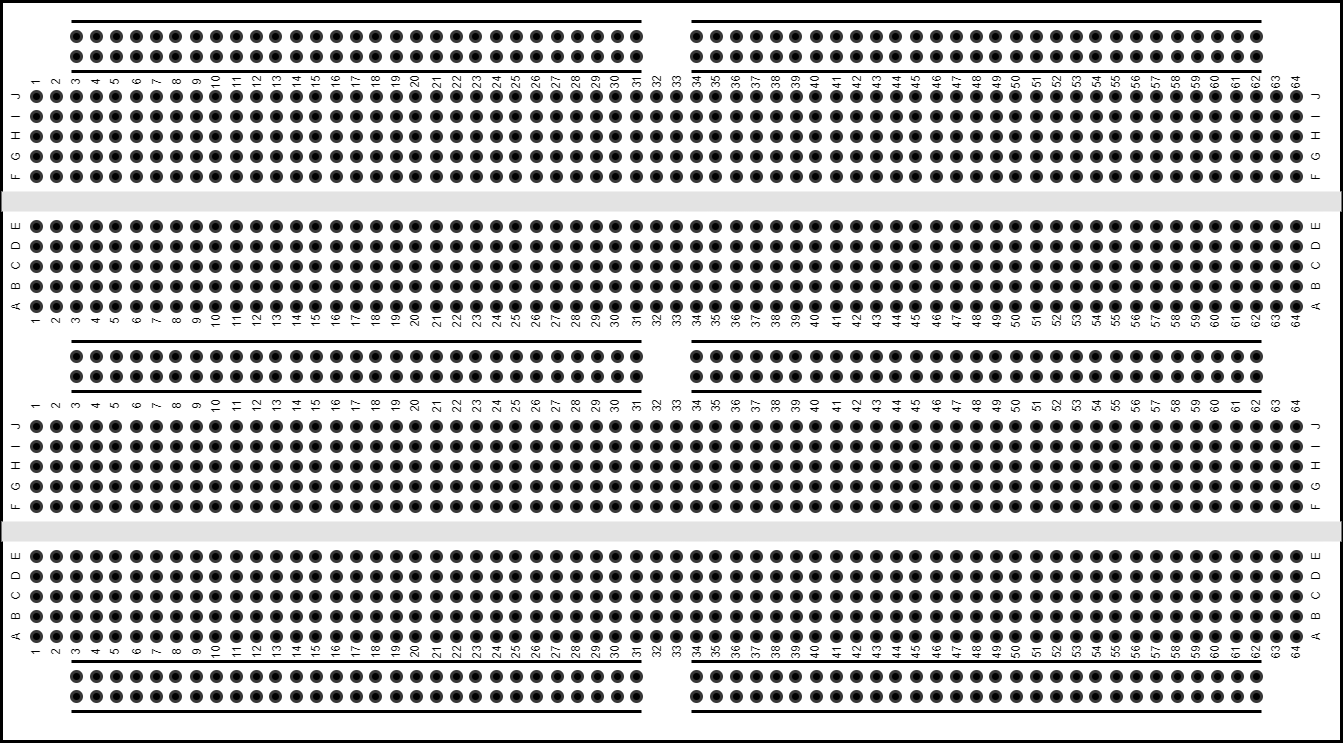
\includegraphics[width=10cm]{./images/breadboard.drawio.png}
  \caption{ブレッドボード}
  \label{fig:breadboard}
\end{figure}
このブレッドボードは5個の部品に分かれており、2この穴が縦に空いてる場所が3個ある。それの間に10個の穴が縦に空いて真ん中に溝がある部品がある。
3個ある横長の部品は内部で電気的に横につながっており、それは青色と赤色の線が横に書いてある穴同士がつながっている。
個の基板では横に2本の線があるので真ん中のピン同士の電気的なつながりはない。この部品は主に電源の端子として使用される。
今回は青色の線が描かれているところを$GND$、赤色の線が描かれているところを$+5V$として使用する。
2個ある長方形の部品は縦にショートしており、5個の穴が内部で電気的につながっている。真ん中の溝で電気的なつながりは切れている。
そのためこのブレッドボードは縦に5個つながっている穴が縦に4個配置されている。この部品は主にIC、ジャンパ線を挿して回路を作成する部品である。
\subsection{7セグメントLED}
7セグメントLEDは7つのLEDを組み合わせたもので、数字を表示させる用途で使用する。7つのLEDはそれぞれaからgまでの名前がついており、それぞれのLEDを点灯させることで数字を表示させる。
7セグメントLEDの略図を図\ref{fig:7seg}に示す。基本的に一番上から時計回りにaからgまでのLEDが配置されている。
\begin{figure}[h]
  \centering
  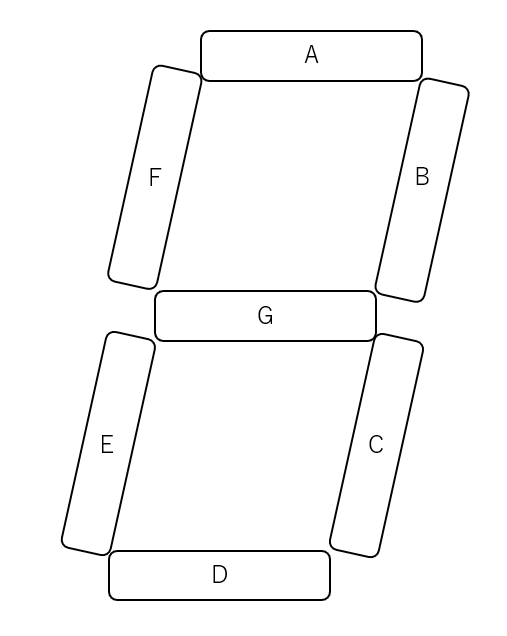
\includegraphics[width=5cm]{./images/7seg.png}
  \caption{7セグメントLEDの略図}
  \label{fig:7seg}
\end{figure}
今回使用するLEDはアノードコモン型の7セグLEDを使用する。アノードコモン型では、その名の通りLEDのアノード端子が共有になっている。
LEDのアノードとは、電流が入力される方向の端子であり、電流を出力する端子をカソードという。アノードからカソードに電流を流すことによりLEDを光らせることが出来る。
そのため、7セグLEDの各LEDの端子とアノードコモンのピンで電圧差が生じたらLEDが光る。アノードコモンのピンには今回は5Vをつなぐため、
各LEDのピンには $GND$ を接続すると光らせることが出来る。
7セグLEDのピン配置を図\ref{fig:7segpin}に示す。
左下のピンから反時計回りに1から10までのピンがあり、3,8がアノードでそれ以外がカソードに接続している。
\begin{figure}[h]
  \centering
  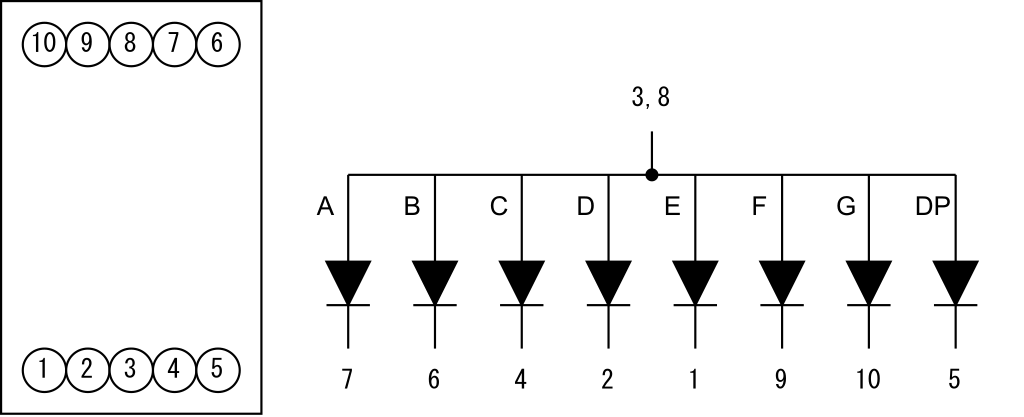
\includegraphics[width=10cm]{./images/7segpin.png}
  \caption{7セグメントLEDのピン配置}
  \label{fig:7segpin}
\end{figure}
\subsection{汎用ロジックIC}
汎用ロジックICでは、論理演算を行うことが出来る回路部品である。2進数の情報を基に7セグLEDの光らせ方を制御するのに使用する。
論理演算ではAND / ORなどがある。例えばAND演算では2本の信号がHIGH($+5V$)の時に出力がHIGHになる。これはどちらも1であるためである。
論理回路の入力と出力を示したものを真理値表という。表の列の数だけ変数があり、入力/出力、場合によっては内部の状態を示す。
AND、OR、NOT、XORの真理値表を表\ref{tab:logic}に示す。今回ではA、Bが入力で、AND、OR、NOT、XOR、が出力である。
この0 1はそれぞれLOW($GND$)、HIGH($+5V$)を示している。
\begin{table}[h]
  \centering
  \caption{論理演算の真理値表}
  \begin{tabular}{|c|c|c|c|c|c|c|}
    \hline
    A & B & AND & OR & NOT (A) & NOT (B) & XOR \\
    \hline
    0 & 0 & 0 & 0 & 1 & 1 & 0 \\
    0 & 1 & 0 & 1 & 1 & 0 & 1 \\
    1 & 0 & 0 & 1 & 0 & 1 & 1 \\
    1 & 1 & 1 & 1 & 0 & 0 & 0 \\
    \hline
  \end{tabular}
  \label{tab:logic}
\end{table}
ICでは内部の特徴に違いがあり、それを名前で表している。今回使用するICは74LSシリーズである。
74LSシリーズはバイポーラトランジスタを使用している。
\textbf{ICの出力端子}
ICには論理回路に入出力があるように、入出力するための端子がある。その内部の構造として、出力端子を説明する。
ICの内部は複数のトランジスタで構成されている。
トランジスタとはスイッチのようなもので、ベースとエミッタの電位差によってコレクタとエミッタ間の電流を制御できる。
トランジスタにはNPN型とPNP型の2種類があるが今回はNPN型で説明を行う。
NPN型トランジスタの特性はベースとエミッタ間に電流が流れる、ようは電位がベースのほうが大きくなるとコレクタからエミッタにかけて電流が流れる。
図 \ref{fig:transistor}では、Bをベース、Cをコレクタ、Eをエミッタとしている。
図 \ref{fig:transistor}(a)にICの出力端子の一個前のイラストを示す。右側の四角いでっぱりが出力端子で内部に書かれているものが出力の一個前のトランジスタである。
図 \ref{fig:transistor}(b)にトランジスタの特性を示す。ベースとエミッタ間に電流が流れるとコレクタとエミッタ間に電流が流れる。そのため出力端子に電流が流れないため、出力はLOWとなる。
この出力の先に電流が流れるかもしれないが、この先に接続するICの内部抵抗よりもトランジスタの抵抗のほうが小さいのでエミッタに電流が流れる。
図 \ref{fig:transistor}(c)では、ベースとエミッタが同じ電位にあるため、コレクタからエミッタにかけて電流が流れない。そのため出力端子の先に違う電位があれば電流が流れる。
IC内部で発生するこれらの電流のことを前者をシンク電流、後者をソース電流という。
\begin{figure}[h]
  \centering
  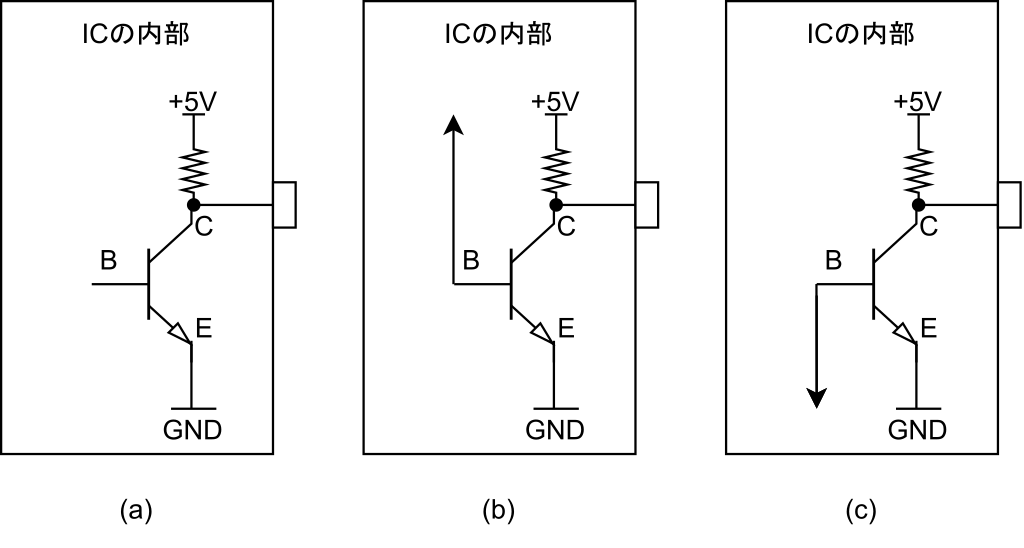
\includegraphics[width=10cm]{./images/trans.png}
  \caption{トランジスタの特性}
  \label{fig:transistor}
\end{figure}
ICによってシンク電流、ソース電流の値が異なるのでデータシートで確認を行い、電子回路を組むことが出来るのかを把握する必要がある。
例えば今回ではアノードコモンのLEDを制御するため出力端子にLEDのカソードを接続し、シンク電流を流すことでLEDを光らせる。
そのため、$I_{ol}$の電流を確認する必要がある。$I_{ol}$はシンク電流、$I_{oh}$はソース電流である。
\textbf{ICの入力端子}
汎用ロジックICではピン番号が同じように命名されている。今回使用するICは74LS04(NOT)、74LS08(AND)、74LS32(OR)、74LS86である。
いずれも14ピンのDIP型のICである。DIPとはDual Inline Packageの略称であり、パッケージの表面にくぼみがあるのが特徴である。
このくぼみがあるほうを表、端子が出てるほうが裏である。表の状態でくぼみを上にした時に、左上から反時計回りに1から14までの数字が命名されている。
74シリーズでは7番に$GND$、14番に$+5V$を接続する。それ以外の端子は入出力端子である。
\subsection{ピンヘッダ}
ピンヘッダを用いて、2進数から10進数に変換する基盤とブレッドボードを接続する。
今回使うピンヘッダは$2\times 7$、端子間距離が$2.54mm$である。
これは一般的なピンヘッダの端子間距離であり今回使用するブレッドボードもこの端子間距離である。
2列のピンヘッダをブレッドボードにそのまま刺すと、2つのピンがショートしてしまうため、T字型コネクタを用いる。
\subsection{カルノー図}
デコーダ回路は複雑な回路になるため、論理式を立てる。論理式は真理値表を基に作成することが出来るが、複雑な回路になると論理式が複雑になる。
そのため、カルノー図を使用することで論理式を簡単に作成することが出来る。
カルノー図は出力の数だけ表を作成し、論理式の作成を行う。表 \ref{tab:karno}にカルノー図の例を示す。
これは7セグLEDのB端子用のカルノー図である。真理値表からここから論理式の計算を行う。
まず初めに、表の中で1の部分をグループ化を行う。その後、グループ化した部分を論理式に変換する。
グループ化したものを\ref{fig:karno1}に示す。これを論理式に変換すると 数式\eqref{eq:b-output} となる。
これを簡単にすると、 \eqref{eq:b-output1} となる。6個の論理素子の使用から、3個の論理素子の使用に減らすことが出来る。
カルノー図から論理式を立てて簡略化してないように見えるが真理値表から論理式を立てた場合、出力がHIGHの量の数 $\times$  3個の論理素子が必要になる式になる。
そのため今回ではカルノー図にする前は30個の論理素子が必要であった。

\begin{figure}[htbp]
  \begin{minipage}[b]{0.49\columnwidth}
  \centering
  \askmapiv{\(B\)}{{\(EN\)}{\(IN_0\)}{\(IN_1\)}{\(IN_2\)}}{}{1111 1111 {\phantom{0}}{\phantom{0}}{\phantom{0}}{\phantom{0}} {\phantom{0}}11{\phantom{0}}}{}
  \caption{\(B\)のカルノー図}
  \label{}
  \end{minipage}
  \begin{minipage}[b]{0.49\columnwidth}
  \centering
  \askmapiv{\(B\)}{{\(EN\)}{\(IN_0\)}{\(IN_1\)}{\(IN_2\)}}{}{11111111{\phantom{0}}{\phantom{0}}{\phantom{0}}{\phantom{0}}{\phantom{0}}11{\phantom{0}}}
  {
   \color{black}\put(0.85,2){\oval(1.8,3.8)}
   \color{black}\put(1.9,2.5){\oval(1.8,0.8)}
   \color{black}\put(1.9,0.5){\oval(1.8,0.8)}
  }
  \caption{\(B\)のカルノー図}
  \label{fig:karno1}
  \end{minipage}
\end{figure}


\section{実験方法}
\subsection{論理式の作成}
デコーダ回路の回路図を作成するために真理値表を作成して論理式を立てていく。
作成した真理値表を表\ref{tab:truth}に示す。この真理値表を元にカルノー図を作成し、論理式を立ててセグメントごとの回路図を作成する。
\begin{table}[h]
  \centering
  \caption{真理値表}
  \begin{tabular}{|c|c|c|c|c|c|c|c|c|c|c|}
    \hline
    $EN$ & $IN_2$ & $IN_1$ & $IN_0$ & $A$ & $B$ & $C$ & $D$ & $E$ & $F$ & $G$ \\
    \hline
    0 & * & * & * & 1 & 1 & 1 & 1 & 1 & 1 & 1 \\
    1 & 0 & 0 & 0 & 0 & 0 & 0 & 0 & 0 & 0 & 1 \\
    1 & 0 & 0 & 1 & 1 & 0 & 1 & 1 & 1 & 1 & 0 \\
    1 & 0 & 1 & 0 & 0 & 0 & 0 & 0 & 0 & 1 & 0 \\
    1 & 0 & 1 & 1 & 0 & 0 & 0 & 0 & 1 & 1 & 0 \\
    1 & 1 & 0 & 0 & 1 & 0 & 0 & 1 & 1 & 0 & 0 \\
    1 & 1 & 0 & 1 & 0 & 1 & 0 & 0 & 1 & 0 & 0 \\
    1 & 1 & 1 & 0 & 0 & 1 & 0 & 0 & 0 & 0 & 0 \\
    1 & 1 & 1 & 1 & 0 & 0 & 0 & 1 & 1 & 0 & 1 \\
    \hline
  \end{tabular}
  \label{tab:truth}
\end{table}
\\
\subsection{セグメントB}
セグメント$B$のカルノー図を図 \ref{fig:karnoB}に示す。このカルノー図を基に作成した式を数式\eqref{eq:b-output}に示す。これを基に作成したセグメントBの回路図を図\ref{fig:segB}に示す。
\begin{figure}[htbp]
  \centering
  \askmapiv{\(B\)}{{\(EN\)}{\(IN_2\)}{\(IN_1\)}{\(IN_0\)}}{}{11111111{\phantom{0}}{\phantom{0}}{\phantom{0}}{\phantom{0}}{\phantom{0}}11{\phantom{0}}}
  {
   \color{black}\put(0.85,2){\oval(1.8,3.8)}
   \color{black}\put(1.9,2.5){\oval(1.8,0.8)}
   \color{black}\put(1.9,0.5){\oval(1.8,0.8)}
  }
  \caption{\(B\)のカルノー図}
  \label{fig:karnoB}
\end{figure}

\begin{align}
  B &= \overline{EN} + IN_0 \cdot \overline{IN_1} \cdot IN_2 + \overline{IN_0} \cdot IN_1 \cdot IN_2 \label{eq:b-output}\\
  &= \overline{EN} + IN_2 \cdot (IN_0 \oplus IN_1  ) \label{eq:b-output1}
\end{align}

\begin{figure}[htbp]
  \centering
  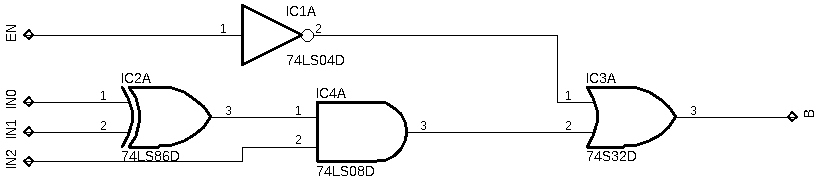
\includegraphics{./images/B.png}
  \label{fig:segB}
  \caption{セグメントBの回路図}
\end{figure}
\newpage
\subsection{セグメントC}
セグメント$C$のカルノー図を図 \ref{fig:karnoC}に示す。このカルノー図を基に作成した式を数式\eqref{eq:c-output}に示す。これを基に作成したセグメントCの回路図を図\ref{fig:segC}に示す。
\begin{figure}[htbp]
  \centering
  \askmapiv{\(C\)}{{\(EN\)}{\(IN_2\)}{\(IN_1\)}{\(IN_0\)}}{}{11111111{\phantom{0}}1{\phantom{0}}{\phantom{0}}{\phantom{0}}{\phantom{0}}{\phantom{0}}{\phantom{0}}}
  {
   \color{black}\put(0.85,2){\oval(1.8,3.8)}
   \color{black}\put(3.9,2.5){\oval(1.8,0.8)[l]}
   \color{black}\put(-0.1,2.5){\oval(1.8,0.8)[r]}
  }
  \caption{\(C\)のカルノー図}
  \label{fig:karnoC}
\end{figure}

\begin{align}
  C &= \overline{EN} + \overline{IN_2} \cdot IN_1 \cdot \overline{IN_0}\label{eq:c-output}
\end{align}

\begin{figure}[htbp]
  \centering
  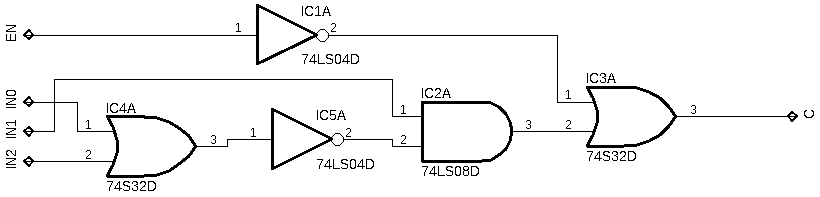
\includegraphics{./images/C.png}
  \label{fig:segC}
  \caption{セグメントCの回路図}
\end{figure}
\newpage
\subsection{セグメントD}
セグメント$D$のカルノー図を図 \ref{fig:karnoD}に示す。このカルノー図を基に作成した式を数式\eqref{eq:d-output}に示す。これを基に作成したセグメントDの回路図を図\ref{fig:segD}に示す。
\begin{figure}[htbp]
  \centering
  \askmapiv{\(D\)}{{\(EN\)}{\(IN_2\)}{\(IN_1\)}{\(IN_0\)}}{}{11111111{\phantom{0}}1{\phantom{0}}{\phantom{0}}1{\phantom{0}}{\phantom{0}}1}{
  \color{black}\put(0.85,2){\oval(1.8,3.8)}
  \color{black}\put(3.9,2.5){\oval(1.8,0.8)[l]}
  \color{black}\put(-0.1,2.5){\oval(1.8,0.8)[r]}
  \color{black}\put(1.9,3.5){\oval(1.8,0.8)}
  \color{black}\put(1.9,1.5){\oval(1.8,0.8)}
}
\caption{\(D\)のカルノー図}
\label{fig:karnoD}
\end{figure}
\begin{align}
  D &= \overline{EN} + IN_2 \cdot IN_1 \cdot IN_0 + IN_2 \cdot \overline{IN_1} \cdot \overline{IN_0} + \overline{IN_2} \cdot \overline{IN_1} \cdot IN_0\label{eq:d-output}\\
  &= \overline{EN} + IN_1 \cdot (IN_2 \oplus IN_0) + IN_2 \cdot IN_1 \cdot IN_0\label{eq:d-output1}
\end{align}
\begin{figure}[htbp]
  \centering
  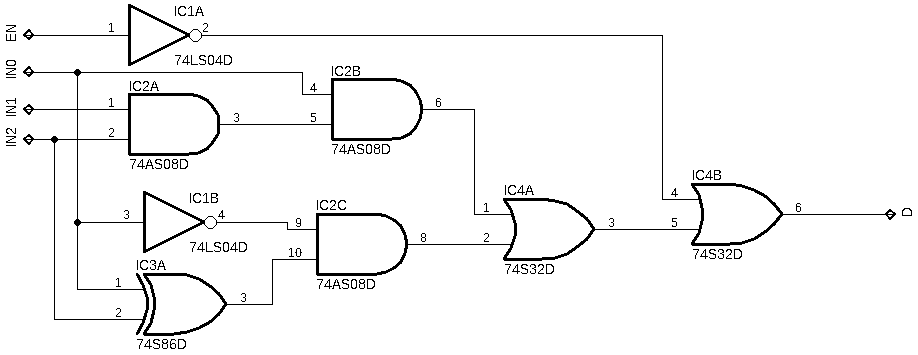
\includegraphics{./images/D.png}
  \label{fig:segD}
  \caption{セグメントDの回路図}
\end{figure}
\newpage
\subsection{セグメントE}
セグメント$E$のカルノー図を図 \ref{fig:karnoE}に示す。このカルノー図を基に作成した式を数式\eqref{eq:e-output}に示す。これを基に作成したセグメントEの回路図を図\ref{fig:segE}に示す。
\begin{figure}[htbp]
  \centering
    \askmapiv{\(E\)}{{\(EN\)}{\(IN_2\)}{\(IN_1\)}{\(IN_0\)}}{}{11111111{\phantom{0}}1{\phantom{0}}111{\phantom{0}}1}{
      \color{black}\put(0.85,2){\oval(1.8,3.8)}
      \color{black}\put(1.9,2.0){\oval(3.8,1.8)}
      \color{black}\put(1.9,3.0){\oval(1.8,1.8)}
    }
    \caption{\(E\)のカルノー図}
    \label{fig:karnoE}
\end{figure}
\begin{align}
  E &= \overline{EN} + IN_0 + \overline{IN_1} \cdotp IN_2\label{eq:e-output}
\end{align}
\begin{figure}[htbp]
  \centering
  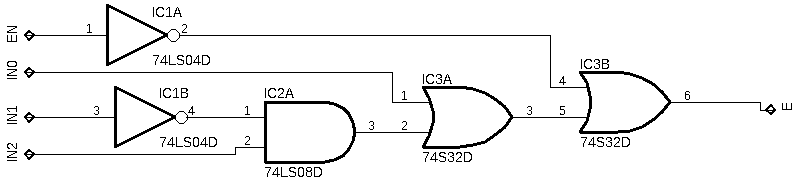
\includegraphics{./images/E.png}
  \label{fig:segE}
  \caption{セグメントEの回路図}
\end{figure}
\newpage
\subsection{セグメントF}
セグメント$F$のカルノー図を図 \ref{fig:karnoF}に示す。このカルノー図を基に作成した式を数式\eqref{eq:f-output}に示す。これを基に作成したセグメントFの回路図を図\ref{fig:segF}に示す。
\begin{figure}[htbp]
  \centering
  \askmapiv{\(F\)}{{\(EN\)}{\(IN_2\)}{\(IN_1\)}{\(IN_0\)}}{}{11111111{\phantom{0}}1{\phantom{0}}{\phantom{0}}1{\phantom{0}}1}{
    \color{black}\put(0.85,2){\oval(1.8,3.8)}
    \color{black}\put(3.9,2.5){\oval(1.8,0.8)[l]}
    \color{black}\put(-0.1,2.5){\oval(1.8,0.8)[r]}
    \color{black}\put(1.9,4.0){\oval(1.8,1.8)[b]}
    \color{black}\put(1.9,0.0){\oval(1.8,1.8)[t]}
  }
  \caption{\(F\)のカルノー図}
  \label{fig:karnoF}
\end{figure}
\begin{align}
  F &= \overline{EN} + IN_0 \cdot \overline{IN_2} + IN_1 \cdot \overline{IN_2}\label{eq:f-output}\\
  &= \overline{EN} + \overline{IN_2} \cdot (IN_0 + IN_1) \label{eq:f-output1}
\end{align}
\begin{figure}[htbp]
  \centering
  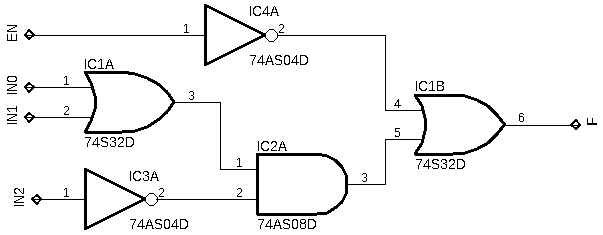
\includegraphics{./images/F.png}
  \label{fig:segF}
  \caption{セグメントFの回路図}
\end{figure}
\newpage
\subsection{セグメントG}
セグメント$G$のカルノー図を図 \ref{fig:karnoG}に示す。このカルノー図を基に作成した式を数式\eqref{eq:g-output}に示す。これを基に作成したセグメントGの回路図を図\ref{fig:segG}に示す。
\begin{figure}[htbp]
  \centering
  \askmapiv{\(G\)}{{\(EN\)}{\(IN_2\)}{\(IN_1\)}{\(IN_0\)}}{}{111111111{\phantom{0}}{\phantom{0}}{\phantom{0}}{\phantom{0}}{\phantom{0}}{\phantom{0}}1}{
    \color{black}\put(0.85,2){\oval(1.8,3.8)}
    \color{black}\put(3.9,3.5){\oval(1.8,0.8)[l]}
    \color{black}\put(-0.1,3.5){\oval(1.8,0.8)[r]}
    \color{black}\put(1.9,1.5){\oval(1.8,0.8)}
  }
  \caption{\(G\)のカルノー図}
  \label{fig:karnoG}
\end{figure}
\begin{align}
  G &= \overline{EN} + \overline{IN_2} \cdot \overline{IN_1}+ IN_2 \cdot IN_1 \cdot IN_0\label{eq:g-output}
\end{align}
\begin{figure}[htbp]
  \centering
  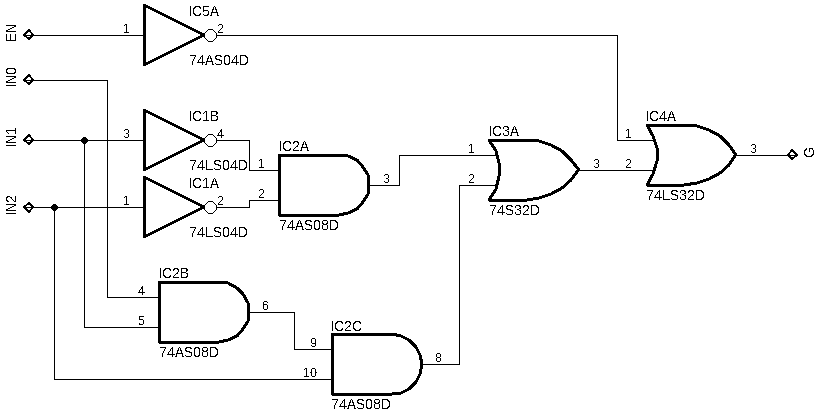
\includegraphics{./images/G.png}
  \label{fig:segG}
  \caption{セグメントGの回路図}
\end{figure}

\newpage
\subsection{ブレッドボードへの配線}
作成した回路図を基にブレッドボードへの配線を行う。使用する部品を表\ref{tab:parts}に示す。
\begin{figure}[htbp]
  \centering
  \begin{tabular}{|c|c|c|}
    \hline
    部品名 & 数量 & 用途 \\
    \hline
    ブレッドボード & 1 & 配線用部品 \\
    74LS04 & 2 & NOT回路 \\
    74LS08 & 2 & AND回路 \\
    74LS32 & 4 & OR回路 \\
    74LS86 & 2 & XOR回路 \\
    7セグLED & 1 & 表示部品 \\
    ピンヘッダ & 1 & ブレッドボードと基盤の接続 \\
    ブレッドボード & 1 & 配線用部品 \\
    エンコーダ回路 & 1 & 2進数から10進数への変換 \\
    抵抗(380 $\Omega$) & 7 & 7セグLEDの入力電流制御 \\
    \hline
  \end{tabular}
  \caption{使用部品}
  \label{tab:parts}
\end{figure}
\subsection{動作確認}
デコード回路が正しく動作しているかの確認に動作確認基盤を用いる。
これはピンヘッダを用いてブレッドボードに接続する部品で、2進数の出力を行うことが出来る。
この基盤を用いて、2進数の入力を行い、7セグLEDが正しく表示されるか確認を行う。
\newpage
\section{結果}
作成した回路をブレッドボードに配線を行い、LEDが正常に点灯することを確認した。入力と出力の関係を表\ref{tab:input-output}に示す。
\begin{table}[h]
  \centering
  \caption{入力と出力の関係}
  \begin{tabular}{|c|c|c|c|c|}
    \hline 
    \rm $(0)_{10}$ & \rm $(1)_{10}$ & \rm $(2)_{10}$ & \rm $(3)_{10}$ & \rm $(4)_{10}$ \\
    \hline
    \begin{minipage}{0.15\columnwidth}
      \centering
      \scalebox{0.15}{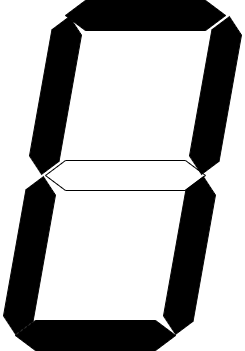
\includegraphics{./images/7seg0.drawio.png}}
    \end{minipage} &
    \begin{minipage}{0.15\columnwidth}
      \centering
      \scalebox{0.15}{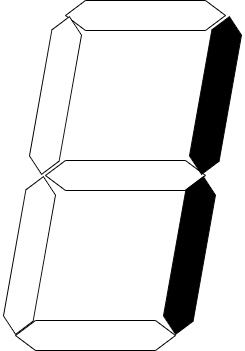
\includegraphics{./images/7seg1.drawio.png}}
    \end{minipage} &
    \begin{minipage}{0.15\columnwidth}
      \centering
      \scalebox{0.15}{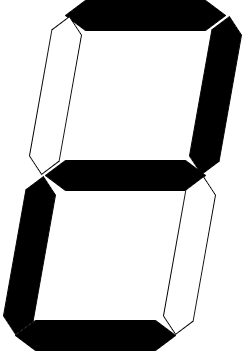
\includegraphics{./images/7seg2.drawio.png}}
    \end{minipage} &
    \begin{minipage}{0.15\columnwidth}
      \centering
      \scalebox{0.15}{
\includegraphics{./images/7seg3.drawio.png}}
    \end{minipage} &
    \begin{minipage}{0.15\columnwidth}
      \centering
      \scalebox{0.15}{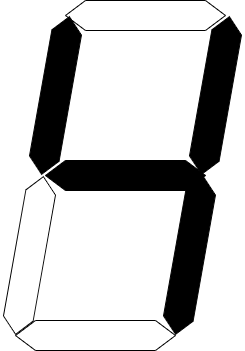
\includegraphics{./images/7seg4.drawio.png}}
    \end{minipage} \\
    \hline
    \rm $(5)_{10}$ & \rm $(6)_{10}$ & \rm $(7)_{10}$ & \rm $EN_{on}$ & \rm $EN_{off}$ \\
    \hline
    \begin{minipage}{0.15\columnwidth}
      \centering
      \scalebox{0.15}{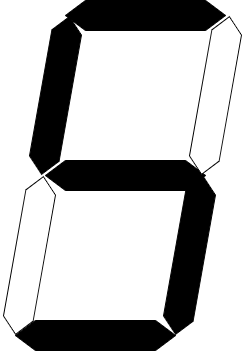
\includegraphics{./images/7seg5.drawio.png}}
    \end{minipage} &
    \begin{minipage}{0.15\columnwidth}
      \centering
      \scalebox{0.15}{
\includegraphics{./images/7seg6.drawio.png}}
    \end{minipage} &
    \begin{minipage}{0.15\columnwidth}
      \centering
      \scalebox{0.15}{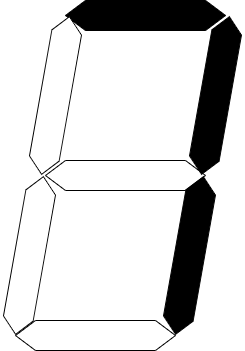
\includegraphics{./images/7seg7.drawio.png}}
    \end{minipage} &
    \begin{minipage}{0.15\columnwidth}
      \centering
      \scalebox{0.15}{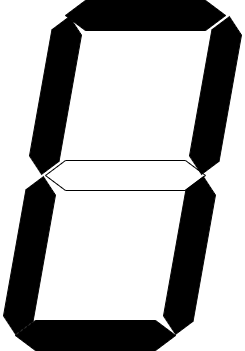
\includegraphics{./images/7segen.drawio.png}}
    \end{minipage} &
    \begin{minipage}{0.15\columnwidth}
      \centering
      \scalebox{0.15}{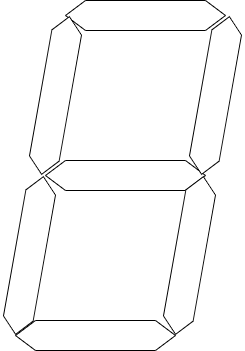
\includegraphics{./images/7seg.drawio.png}}
    \end{minipage} \\
    \hline
  \end{tabular} 
  \label{tab:input-output}
\end{table}
\section{報告事項}
  \subsection{$VCC = 5[V]$の電源を使って$I_f = 8[mA]$、$V_f = 1.98[V]$のLEDを適切に光らせるには、抵抗の値をいくらにすればよいか。}
  $ R = \frac{VCC - V_f}{I_f} = \frac{5 - 1.98}{0.008} = 377.5[\Omega]$より、$380[\Omega]$の抵抗を使用する。
  \subsection{バイポーラトランジスタとCOMSの特徴を調べて報告してください。}
  バイポーラトランジスタにはPNP型とNPN型があり、NPN型はPNP型と逆の特性を持っている。
  NPN型ではベースからエミッタにかけて電流が流れるとコレクタからエミッタにかけて電流が流れる。
  そして、ベースからエミッタにかけて流れる電流はコレクタからエミッタにかける電流よりも小さいため、電流の増幅を行うことが出来る。
  CMOSは、MOSFETを用いた回路である。MOSFETとはバイポーラトランジスタと違いゲートに電圧を印加することによりチャネルを形成し、電流を流すことが出来る。
  そのため一度駆動してしまえば電流の消費が少ないため駆動しているときの消費電力が少ない。
  \subsection{ファンイン、ファンアウトについて調べて報告してさい}
  ファンイン、ファンアウトとは論理素子の入力端子、出力端子の数のことを言う。\\
  バイポーラトランジスタで構成されているICの場合、シンク電流やソース電流によって同じ配線で次に駆動できるICの数が決まる。
  例えば $I_{ol} = 0.4[mA]$、 $ I_{il} = 0.1[mA]$の場合、$I_{ol} = I_{il} \times n$より、$n = 4$となる。この同時に接続できる数がファンアウトである。
  ファンインとは、ICの入力端子に接続できる数のことである。
  \subsection{表2.2にある真理値表を完成させてください}
  表\ref{tab:truth}に真理値表を示す。
  \subsection{7セグメントLEDおよび抵抗を含めた、すべてのセグメントをまとめた回路図を描いてください}
  7セグメントLEDおよび抵抗を含めた、すべてのセグメントをまとめた回路図を図\ref{fig:circit}に示す。
  \begin{figure}[htbp]
    \centering
    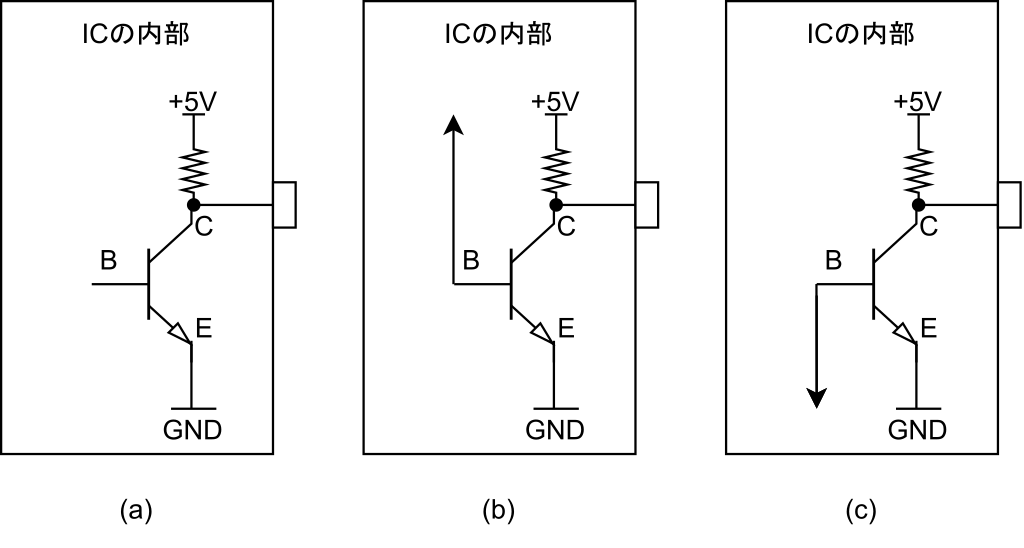
\includegraphics[angle = 90,width = 0.95\columnwidth]{./images/circit.png}
    \caption{7セグメントLEDの回路図}
    \label{fig:circit}
  \end{figure}
  \newpage
  \section{考察}
今回の実験では、7セグメントLEDを制御するための回路を作成することが出来た。
論理回路を組むときにカルノー図を使用すると簡単化を行えて、回路をより簡単なものにすることが出来た。


\end{document}